\documentclass[tikz]{standalone}

\begin{document}
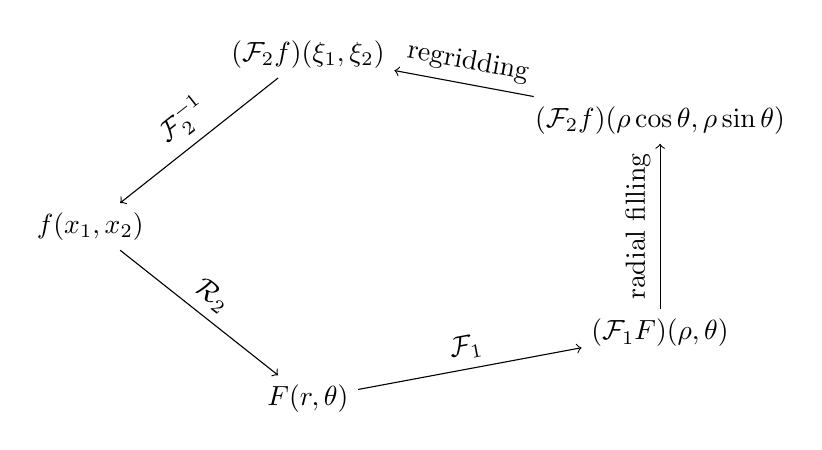
\begin{tikzpicture}
	\def\rad{3.5}
	\foreach [count=\i] \name/\labl in {
		obj/{f(x_1, x_2)},
		radon/{F(r,\theta)},
		fourier radon/{(\mathcal{F}_1F)(\rho, \theta)},
		radial fourier/{(\mathcal{F}_2 f)(\rho\cos\theta, \rho\sin\theta)},
		cartesian fourier/{(\mathcal{F}_2 f)(\xi_1, \xi_2)}
	}
	{
		\node (\name) at ({4*cos(180+72*\i-72)}, {2.3*sin(180+72*\i-72)}) {\( \labl \)};
	}
	\foreach \no/\nt/\labl in {
		obj/radon/{\( \mathcal{R}_2 \)},
		radon/fourier radon/{\( \mathcal{F}_1 \)},
		fourier radon/radial fourier/{radial filling},
		radial fourier/cartesian fourier/{regridding},
		cartesian fourier/obj/{\( \mathcal{F}_2^{-1} \)}
	}
	{
		\draw [->] (\no) -- (\nt) node [midway, sloped, above] {\labl};
	}
\end{tikzpicture}
\end{document}
